% =====================================================================
% AI Academy -- National AI Center
% Software Engineering Final Project -- Team Report Template
%
% HOW TO USE
% ----------
%   1. Edit the CONFIGURATION block below (team name, topic, members).
%   2. Replace every [TODO: ...] with your content. TODOs render in red,
%      so anything you forgot will be visually obvious in the PDF.
%   3. Three kinds of cues throughout:
%        - REQUIRED DELIVERABLE box (blue): exactly what we expect.
%        - PROBING QUESTIONS box (amber): NOT a checklist; these are
%          prompts that should shape how you write the section. A strong
%          response engages with at least 2 of them; a weak response
%          ignores them all.
%        - "Your response:" placeholders: replace with your text/diagram.
%   4. Target length: 8-10 pages including figures, excluding bibliography.
%   5. Compile with pdfLaTeX. Overleaf works out of the box.
% =====================================================================

\documentclass[11pt,a4paper]{article}

% ===== EARLY MACROS (must come before configuration) =================
% (Full styling lower down; we just need \TODO and \ph available
% before the configuration block uses them.)
\usepackage[dvipsnames]{xcolor}
\definecolor{accent2}{HTML}{8B0000}
\definecolor{ph}{HTML}{6B7280}
\newcommand{\TODO}[1]{\textcolor{accent2}{\textbf{[TODO: #1]}}}
\newcommand{\phh}[1]{\textcolor{ph}{\textit{#1}}}

% ===== CONFIGURATION (edit these) ====================================
\newcommand{\teamname}{Team\_3\_M503}
\newcommand{\topicchoice}{Topic 2 -- AI Food Analyzer}
\newcommand{\member}[2]{\textbf{#1} (#2)}  % name, GitHub handle
\newcommand{\reportdate}{Sept. 19, 2026}
\newcommand{\repolink}{\url{https://github.com/atlukhanovmurad2-ui/swe_project}}

% ===== course meta (rarely changes) ==================================
\newcommand{\coursecode}{AI-ENG-110}
\newcommand{\coursename}{Software Engineering}
\newcommand{\institution}{AI Academy, National AI Center}
\newcommand{\semester}{Spring 2026}

% ===== PACKAGES ======================================================
\usepackage[margin=2.2cm,headheight=15pt]{geometry}
\usepackage[T1]{fontenc}
\usepackage[utf8]{inputenc}
\usepackage[final,protrusion=true,expansion=false]{microtype}
\usepackage{amsmath,amssymb}
\usepackage{graphicx}
\usepackage{booktabs}
\usepackage{array}
\usepackage{tabularx}
\usepackage{ragged2e}
\usepackage{enumitem}
\usepackage[parfill]{parskip}
\usepackage{listings}
\usepackage[most]{tcolorbox}
\usepackage{titlesec}
\usepackage{fancyhdr}
\usepackage{lastpage}
\usepackage[hidelinks]{hyperref}
\usepackage{tikz}
\usetikzlibrary{arrows.meta,positioning,fit}

\emergencystretch=3em
\hbadness=10000
\hfuzz=2pt

\hypersetup{
  colorlinks=true,
  linkcolor=NavyBlue,
  urlcolor=NavyBlue,
  citecolor=NavyBlue,
  pdftitle={\coursecode\ Final Project Report},
  pdfauthor={\teamname}
}

% ===== STYLING =======================================================
\definecolor{accent}{HTML}{0B3D91}
\definecolor{soft}{HTML}{F2F4F8}
\definecolor{deliver}{HTML}{E8F0FE}
\definecolor{deliverframe}{HTML}{1A56DB}
\definecolor{probe}{HTML}{FFF8E1}
\definecolor{probeframe}{HTML}{B45309}

\titleformat{\section}
  {\Large\bfseries\color{accent}}{\thesection.}{0.6em}{}
\titleformat{\subsection}
  {\large\bfseries\color{accent}}{\thesubsection}{0.5em}{}

\newcommand{\ans}[1]{\rule[-2pt]{#1}{0.5pt}}
\let\ph\phh  % alias the early \phh as \ph for consistency with the body

% Deliverable callout (light blue)
\newtcolorbox{deliverbox}{
  colback=deliver, colframe=deliverframe, boxrule=0.5pt,
  arc=2pt, left=8pt, right=8pt, top=4pt, bottom=4pt
}
% Probing-question callout (light amber)
\newtcolorbox{probebox}{
  colback=probe, colframe=probeframe, boxrule=0.5pt,
  arc=2pt, left=8pt, right=8pt, top=4pt, bottom=4pt
}

\newcommand{\answerbox}[2]{%
  \par\noindent
  \fcolorbox{black!30}{soft}{%
    \parbox{\dimexpr\linewidth-2\fboxsep-2\fboxrule-30pt\relax}{%
      \vspace{2pt}\raggedright
      #2
      \vspace{2pt}
    }%
  }\par
}

\newcommand{\figureplaceholder}[2]{%
  \par\noindent
  \begin{center}
  \fcolorbox{black!30}{soft}{%
    \parbox{0.75\linewidth}{%
      \vspace{2pt}\centering
      #2
      \vspace{2pt}
    }%
  }
  \end{center}
}

\definecolor{codegreen}{rgb}{0,0.55,0}
\definecolor{codegray}{rgb}{0.4,0.4,0.4}
\definecolor{codepurple}{rgb}{0.55,0,0.78}
\definecolor{backcolour}{rgb}{0.97,0.97,0.97}

\lstdefinestyle{python}{
  language=Python,
  backgroundcolor=\color{backcolour},
  commentstyle=\color{codegreen},
  keywordstyle=\color{accent},
  numberstyle=\tiny\color{codegray},
  stringstyle=\color{codepurple},
  basicstyle=\ttfamily\footnotesize,
  breakatwhitespace=false,
  breaklines=true,
  keepspaces=true,
  numbers=left,
  numbersep=6pt,
  tabsize=2,
  frame=single,
  framerule=0.4pt,
  rulecolor=\color{black!30},
}

\pagestyle{fancy}
\fancyhf{}
\fancyhead[L]{\small\textit{\coursecode\ -- Final Report -- \teamname}}
\fancyhead[R]{\small\textit{\semester}}
\fancyfoot[L]{\small\textit{\institution}}
\fancyfoot[R]{\small Page \thepage\ of \pageref{LastPage}}
\renewcommand{\headrulewidth}{0.4pt}
\renewcommand{\footrulewidth}{0.4pt}

% =====================================================================
\begin{document}

\begin{center}
{\small \textsc{\institution} \\[0.2em] \textsc{\coursecode\ -- \coursename\ -- \semester}}\\[1.2em]
{\Large\bfseries\color{accent} Final Project Report}\\[0.3em]
{\LARGE\bfseries \topicchoice}\\[0.6em]
\rule{0.85\textwidth}{0.6pt}
\end{center}

\vspace{0.6em}
\begin{tabularx}{\textwidth}{@{}lXlX@{}}
\textbf{Team:} & \teamname & \textbf{Date:} & \reportdate \\
\textbf{Repo:} & \repolink & \textbf{Tag:} & \texttt{v1.0-final} \\
\textbf{Members:} & \multicolumn{3}{X@{}}{%
  \member{Murad Atlukhanov}{@atlukhanovmurad2-ui},\quad
  \member{Zhala Afandiyeva}{@zhafandiyeva}\quad
  \member{Penah Quliyev}{@pnah6699-maker}\quad
}\\
\end{tabularx}
\vspace{0.4em}\hrule\vspace{0.6em}

% ===== EXECUTIVE SUMMARY =============================================
\section*{Executive Summary}
\addcontentsline{toc}{section}{Executive Summary}

\begin{deliverbox}
\textbf{Required.} Exactly one paragraph (5--7 sentences). What you built, the headline concurrency speedup you measured, your headline robustness story, and the single most surprising thing the team learned. \emph{This is the first thing the grader reads. If you cannot write it clearly, you do not yet understand your own project.}
\end{deliverbox}

\begin{probebox}
\textit{Your paragraph should answer:} What problem did the system solve? What is the one number that proves the concurrency design works? What is the one failure mode you handled well? What would you change if you started over?
\end{probebox}

\answerbox{3cm}{We built an AI Food Analyzer that accepts a meal image and returns ingredients, estimated portions, nutrition values, totals, and a macronutrient split. Users can run it through a CLI or a FastAPI service, while PostgreSQL stores analysis history when configured. Six simulated nutrition requests took 1.206 seconds sequentially and 0.208 seconds concurrently, a 5.8-times speedup. The system validates files, retries provider failures, limits parallel work, and returns partial results when one nutrition lookup fails. Offline providers keep tests repeatable without network access. The most useful lesson was that one failed ingredient should not remove successful results for the rest of the meal. With more time, we would add strict request timeouts and complete 429 handling.}

% ===== TABLE OF CONTENTS =============================================
\tableofcontents
\vspace{0.6em}\hrule\vspace{0.4em}

% =====================================================================
\section{Project Overview}

\subsection{Problem framing \& scope}

\begin{deliverbox}
\textbf{Required.} 2--3 paragraphs. State the topic problem in your own words. List the inputs, outputs, and any user-facing entry points (CLI commands, HTTP endpoints). State which provider stack you used (LLM, embedding, USDA, web search).
\end{deliverbox}

\begin{probebox}
\textit{Beyond the obvious:} which parts of the TOPIC.md spec did your team explicitly decide \emph{not} to do, and why? Where did you tighten the spec? Where did you loosen it?
\end{probebox}

\answerbox{4cm}{The system solves the problem of estimating nutrition from a cooked meal that has no food label. Its input is a JPEG or PNG meal image. Its output contains identified ingredients, estimated grams, calories, protein, carbohydrates, fat, totals, confidence values, and warnings.

The CLI provides \texttt{analyze} and \texttt{history}. The HTTP service provides \texttt{POST /analyze}, \texttt{GET /health}, \texttt{GET /history}, and \texttt{GET /history/\{id\}}. The normal provider stack is a configurable vision-language model and USDA FoodData Central. During development, OpenAI with \texttt{gpt-4o-mini} was used; offline providers support demos and tests.

We did not build user accounts, a web interface, medical advice, or permanent image storage. We tightened the specification by checking file signatures, not only extensions. We also chose to return a partial result when one USDA lookup fails instead of failing the whole request.}

\subsection{Provider choice and the AI module contract}

\begin{deliverbox}
\textbf{Required.} Name the LLM, embedding, and any auxiliary provider you used, and the model identifiers (\texttt{claude-sonnet-4-6}, \texttt{text-embedding-3-small}, etc.). State what \texttt{ai/} functions you call. \emph{Confirm in one sentence that you did not modify the public interface of the provided \texttt{ai/} package.}
\end{deliverbox}

\begin{probebox}
\textit{Push deeper:} how does your code defend against a malformed model response? What happens when the provider returns valid JSON that is semantically wrong (wrong topic enum, negative grams, etc.)?
\end{probebox}

\answerbox{3cm}{The tested setup used \texttt{LLM\_PROVIDER=openai}, \texttt{LLM\_MODEL=gpt-4o-mini}, and \texttt{NUTRITION\_PROVIDER=usda}. This topic does not need an embedding or web-search provider. The SE layer calls \texttt{ai.identify\_ingredients}, \texttt{ai.get\_nutrition\_provider}, and \texttt{ai.compute\_totals}.

Pydantic validates provider output before the main pipeline uses it. The provided ingredient schema rejects empty names, non-positive or extremely large gram estimates, and confidence outside 0--1. SE-layer models forbid unexpected fields. An empty list becomes \texttt{unknown\_meal}. We did not modify the public interface of the provided \texttt{ai/} package.}

% =====================================================================
\section{Architecture}\label{sec:arch}

\subsection{Module map}

\begin{deliverbox}
\textbf{Required.} An architecture diagram (boxes-and-arrows or sequence diagram) showing the main modules and their dependencies. Identify on the diagram: the boundary of the provided \texttt{ai/} package, your service layer that wraps it, your core business logic, your concurrency layer, your storage layer, and your CLI/HTTP entry points.
\end{deliverbox}

\begin{probebox}
\textit{Interpret your own diagram:} which arrows cross the AI-module boundary? Which arrows cross the storage boundary? If you had to swap providers (Anthropic $\to$ OpenAI), how many files would change?
\end{probebox}

\figureplaceholder{6cm}{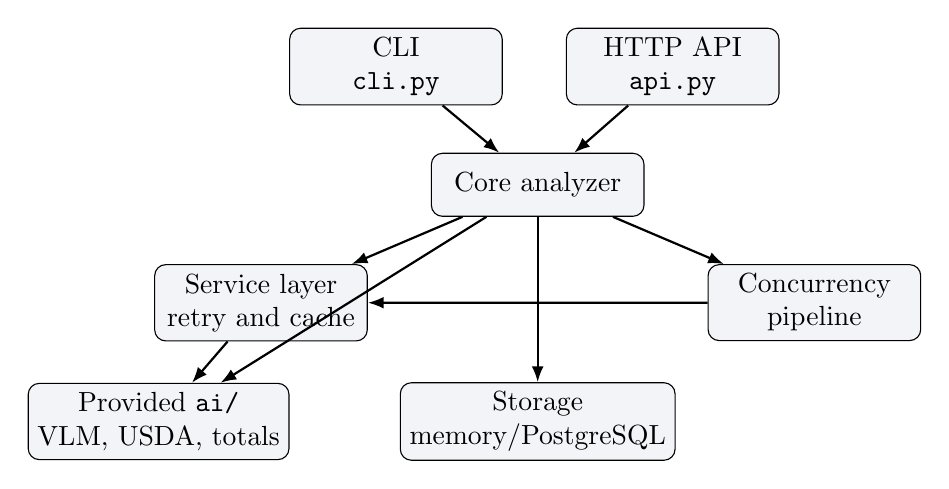
\begin{tikzpicture}[
node distance=6mm and 8mm,
box/.style={draw,rounded corners,align=center,minimum width=27mm,minimum height=8mm,fill=soft},
arr/.style={-{Latex[length=2mm]},thick}]
\node[box] (cli) {CLI\\\texttt{cli.py}};
\node[box,right=of cli] (api) {HTTP API\\\texttt{api.py}};
\node[box,below=of cli,xshift=18mm] (core) {Core analyzer};
\node[box,below left=of core] (service) {Service layer\\retry and cache};
\node[box,below right=of core] (conc) {Concurrency\\pipeline};
\node[box,below=of core,yshift=-15mm] (storage) {Storage\\memory/PostgreSQL};
\node[box,left=of storage,xshift=-6mm] (ai) {Provided \texttt{ai/}\\VLM, USDA, totals};
\draw[arr] (cli)--(core); \draw[arr] (api)--(core);
\draw[arr] (core)--(service); \draw[arr] (core)--(conc);
\draw[arr] (core)--(storage); \draw[arr] (service)--(ai);
\draw[arr] (conc)--(service); \draw[arr] (core)--(ai);
\end{tikzpicture}}

\textbf{Module-by-module summary (1--2 sentences each):} \answerbox{4cm}{The CLI parses commands, selects offline providers when requested, and prints a table or JSON. The API keeps shared settings, storage, and the cached provider during its lifespan. Both call \texttt{analyze\_image}, which controls validation, identification, nutrition lookup, total calculation, and persistence.

The service layer wraps calls that cross into \texttt{ai/} and adds retries, caching, logging, and error translation. The concurrency layer runs independent nutrition lookups in parallel. The storage layer is behind \texttt{HistoryRepository}; arrows into it cross the persistence boundary. Changing Anthropic to OpenAI normally requires only environment changes because provider creation remains behind the factory and wrapper.}

\subsection{OOP design \& key abstractions}

\begin{deliverbox}
\textbf{Required.} Identify at least one example of inheritance or composition \emph{in your own code} (not the provided package's). Quote 5--10 lines of the relevant class or object design. Justify why this abstraction was the right tool; if you used an ABC, explain why.
\end{deliverbox}

\begin{probebox}
\textit{Defensibility:} if a grader asked "why is this an abstract base class rather than a Protocol, a plain function with a callable parameter, or a configuration enum?" --- what is your answer? Are there places where you used composition where inheritance would have been wrong, or vice versa?
\end{probebox}

\textbf{Code listing:}
\begin{lstlisting}[style=python]
class HistoryRepository(abc.ABC):
    @abstractmethod
    async def add(self, record: AnalysisRecord) -> None: ...

    @abstractmethod
    async def list_recent(self, limit: int = 20) -> list[AnalysisRecord]: ...

class PostgresHistoryRepository(HistoryRepository): ...
\end{lstlisting}

\textbf{Justification (2--3 sentences):} \answerbox{2cm}{The abstract class gives the memory and PostgreSQL repositories one asynchronous contract and lets the analyzer depend on behavior instead of database details. A configuration enum would only select a backend and would not define its operations. Composition was better for \texttt{CachingNutritionProvider}: it wraps any provider and adds caching and retries without copying provider code.}

\subsection{Data flow across module boundaries}

\begin{deliverbox}
\textbf{Required.} List the dataclasses you defined for your own SE layer. Confirm in one sentence that no naked dictionaries cross module boundaries.
\end{deliverbox}

\begin{probebox}
\textit{The hardest call:} when did you reuse a dataclass from the provided \texttt{ai/} package vs.\ wrap it in a new one for your SE layer? What was the trigger for wrapping?
\end{probebox}

\answerbox{3cm}{The concurrency layer defines \texttt{LookupOutcome} and \texttt{PipelineResult}. \texttt{RetryPolicy} and the private cache \texttt{\_Entry} are also dataclasses. The SE layer uses Pydantic models for \texttt{AnalysisResult}, \texttt{AnalysisRecord}, \texttt{AnalyzedIngredient}, and \texttt{MacroBreakdown}.

We reuse the provided \texttt{Ingredient} and \texttt{NutritionFacts} while the data belongs to the AI stages. We wrap them when the application needs IDs, timestamps, warnings, storage paths, or per-ingredient status. No naked dictionaries cross the main module boundaries; dictionaries are created only for JSON and database conversion.}

% =====================================================================
\section{Concurrency \& Performance}\label{sec:concurrency}

\subsection{Why this concurrency model}

\begin{deliverbox}
\textbf{Required.} State which concurrency primitive you used (\texttt{asyncio}, \texttt{ProcessPoolExecutor}, \texttt{ThreadPoolExecutor}) and why. Identify the bottleneck the parallel design targets. State the bound (e.g.\ \texttt{Semaphore(10)}) and how you picked it.
\end{deliverbox}

\begin{probebox}
\textit{Justify against alternatives:} could you have used threads instead of asyncio? Why not? What is the smallest workload at which the concurrent design starts to win against sequential? What happens if you set the semaphore to 1 vs.\ 100?
\end{probebox}

\answerbox{4cm}{Nutrition lookup is I/O-bound because each ingredient may require an independent HTTP request. The pipeline uses \texttt{asyncio.gather} and runs the blocking provider call with \texttt{asyncio.to\_thread}. \texttt{Semaphore(10)} is the default bound, and configuration allows 1--100.

A process pool would add unnecessary process cost because the bottleneck is network waiting, not CPU work. Direct threads could work, but asyncio fits FastAPI and asynchronous storage. With a bound of 1, the work becomes effectively sequential. A bound of 100 may trigger provider limits without useful extra speed. Ten is a conservative project default; production tuning needs live load tests and the provider's limits.}

\subsection{Sequential-vs-concurrent benchmark}

\begin{deliverbox}
\textbf{Required.} A table reporting wall-clock time for the same workload run sequentially vs.\ concurrently. State $N$ (number of requests), the machine, the python version, whether caches were cleared, and the command line. Reproduce the table also in your README.
\end{deliverbox}

\begin{probebox}
\textit{Honest interpretation:} did you reach the theoretical $N\times$ speedup? If not, what was the new bottleneck (provider rate limit? GIL? network RTT? single-threaded DB writes?). What would push the curve further?
\end{probebox}

\begin{center}\small
\begin{tabular}{lcccc}
\toprule
\textbf{Workload} & $N$ & \textbf{Sequential (s)} & \textbf{Concurrent (s)} & \textbf{Speedup} \\
\midrule
Simulated nutrition lookups & 6 & 1.206 & 0.208 & 5.8$\times$ \\
\bottomrule
\end{tabular}
\end{center}

\textbf{Discussion (2--3 sentences):} \answerbox{2.5cm}{The benchmark ran with Python 3.13.1 on the team's Windows computer using \texttt{python scripts/benchmark\_pipeline.py}. It used six unique calls with 200 ms simulated latency and no external network or persistent cache. The result is close to 6$\times$ because most time is waiting; thread scheduling and pipeline overhead explain the remaining difference.}

\subsection{Rate limit \& politeness}

\begin{deliverbox}
\textbf{Required.} State the rate-limit strategy (sleep-on-429, token bucket, leaky bucket, request budget). Document the configured budget. State the highest burst your test suite produces.
\end{deliverbox}

\begin{probebox}
\textit{Failure-mode test:} have you actually observed a 429 from the provider during development, or is this strategy untested in anger? What does the log look like when the budget is hit?
\end{probebox}

\answerbox{3cm}{The application limits a batch to 10 concurrent nutrition calls by default. Provider errors are retried up to four times, with delays near 0.5, 1, and 2 seconds plus small jitter. A test sends 12 requests with a bound of 3 and confirms that no more than three are active.

This is not a complete token bucket and does not yet read a \texttt{Retry-After} header. The team tested injected provider failures, not a live 429. Logs include the operation, attempt number, error, and delay. Production code should classify 429 and transient 5xx responses and follow the provider's requested waiting time.}

% =====================================================================
\section{Robustness \& Error Handling}\label{sec:robustness}

\subsection{Wrapping the AI module}

\begin{deliverbox}
\textbf{Required.} Describe your service-layer wrapper around \texttt{ai.*} calls: retries (which exceptions, how many attempts, backoff schedule), timeouts (per-call value), structured logging (what fields, at what level), input validation (what you check before calling, what you check on the response).
\end{deliverbox}

\begin{probebox}
\textit{Pressure-test:} what happens if the provider returns a 500? A 429? A connection reset mid-stream? A perfectly-formed JSON that contradicts the schema? Walk through one of these end-to-end.
\end{probebox}

\answerbox{4cm}{\texttt{services/ai\_service.py} wraps ingredient identification, logs the operation, retries \texttt{ProviderError}, and converts the final failure into \texttt{IngredientIdentificationError}. \texttt{CachingNutritionProvider} applies the same policy to nutrition calls and converts the last provider failure into \texttt{NutritionLookupError}. Defaults are four attempts, 0.5-second base delay, and an 8-second maximum delay.

Before the AI call, the program checks file existence, size, extension, declared type, and JPEG or PNG magic bytes. Pydantic validates structured outputs. INFO logs record stages and timings; WARNING records retries or failed ingredients; ERROR records final failures. Secrets are not logged. The current wrapper has no separate application-level timeout, which is a known gap that should be fixed with timeout-aware HTTP calls.}

\subsection{Failure-mode analysis (one concrete incident)}

\begin{deliverbox}
\textbf{Required.} Pick \emph{one} failure mode you actually exercised (provider 5xx, timeout, malformed response, network drop, disk full, corrupted image, USDA outage, etc.). Describe: (i) how you injected the failure, (ii) what the system did, (iii) what the user saw, (iv) what the logs showed.
\end{deliverbox}

\begin{probebox}
\textit{Go beyond "graceful degradation worked":} what did you originally expect to happen vs.\ what actually happened? Did the test surface any design issue that you then fixed? Did the log give you enough to diagnose it without running the code again?
\end{probebox}

\answerbox{4.5cm}{During a real API run, the VLM identified cooked broccoli, but USDA returned \texttt{403 Forbidden}. The nutrition wrapper retried the provider call and converted the final error into a lookup failure. The concurrency pipeline kept successful ingredients instead of discarding the whole analysis.

The user received HTTP 200 with status \texttt{partial}, the affected item had status \texttt{lookup\_failed}, and a warning explained that totals covered only the remaining ingredients. Logs showed the ingredient, attempts, retry delays, and final failure. We first expected a complete result; the incident showed that provider authentication must be checked separately. It also showed that 403 should fail fast rather than be treated like a temporary error.}

\subsection{Input validation}

\begin{deliverbox}
\textbf{Required.} For every entry point (CLI, HTTP, file, env), list the validation rules. State what error message the user gets when validation fails.
\end{deliverbox}

\begin{probebox}
\textit{Adversarial:} could a malformed image kill your service? A 100\,MB JSON request? A query of 50,000 characters? A path that escapes your storage directory?
\end{probebox}

\answerbox{3cm}{\textbf{CLI:} the path must exist and its content must pass size and magic-byte checks. Errors are printed clearly and return a non-zero exit code. \textbf{HTTP:} \texttt{/analyze} requires one multipart file; empty data, files above 5 MB, unsupported extensions, declared types, or signatures are rejected with structured JSON errors. \textbf{File handling:} the name is sanitized and limited to 60 characters, a UUID is added, and the temporary file is deleted in \texttt{finally}. \textbf{Environment:} Pydantic validates port, concurrency, cache TTL, image size, retry settings, and log level. \textbf{History:} \texttt{limit} is clamped to 1--200 and an unknown ID returns 404. A future version should reject oversized HTTP bodies while streaming instead of reading the full upload first.}

% =====================================================================
\section{Storage \& Caching}\label{sec:storage}

\subsection{Schema}

\begin{deliverbox}
\textbf{Required.} The SQLite schema for your domain tables. Include indices and foreign keys. State which fields are derived (cached) vs.\ source-of-truth.
\end{deliverbox}

\begin{probebox}
\textit{Schema choices:} why did you store embedding bytes as a blob rather than serialized JSON, or vice versa? What happens to the DB if the embedding dimension changes (a different provider, a different model)?
\end{probebox}

\begin{lstlisting}[style=python,language=sql,numbers=none,basicstyle=\ttfamily\small]
CREATE TABLE IF NOT EXISTS analysis_history (
    id             TEXT PRIMARY KEY,
    created_at     TIMESTAMPTZ NOT NULL,
    image_path     TEXT NOT NULL,
    image_filename TEXT NOT NULL,
    status         TEXT NOT NULL,
    ingredients    JSONB NOT NULL,
    totals         JSONB NOT NULL,
    warnings       JSONB NOT NULL DEFAULT '[]'
);
CREATE INDEX IF NOT EXISTS analysis_history_created_at_idx
    ON analysis_history (created_at DESC);
\end{lstlisting}

\subsection{Caching policy}

\begin{deliverbox}
\textbf{Required.} What do you cache, how long, where, and how is the cache invalidated. Report cache hit rate from a demo run (a single number is fine).
\end{deliverbox}

\begin{probebox}
\textit{Correctness vs.\ freshness:} which cached values can become stale (e.g.\ USDA nutrition for a renamed food, an LLM summary if the prompt changes)? How would you detect and evict them in production?
\end{probebox}

\answerbox{2.5cm}{This project uses PostgreSQL, not the generic SQLite example in the template. It caches \texttt{NutritionFacts} in process by normalized ingredient name. The default TTL is 86,400 seconds (24 hours). Entries are removed on expiry, process restart, or an explicit \texttt{invalidate()} call. One repeated-name demo gives one miss followed by one hit, or a 50\% hit rate across two lookups. A meal containing only new names has 0\%. Values may become stale if USDA data or matching rules change; a production key should include provider and matching versions.}

% =====================================================================
\section{Testing}\label{sec:testing}

\subsection{Strategy \& coverage}

\begin{deliverbox}
\textbf{Required.} Report the coverage number (\texttt{pytest --cov}). State how you mocked the AI module and the HTTP layer. Confirm the provided \texttt{tests/test\_ai\_smoke.py} still passes.
\end{deliverbox}

\begin{probebox}
\textit{Quality vs.\ coverage:} which lines did you decide \emph{not} to cover, and why? Which mocks did you have to redesign mid-project because they were testing the wrong thing?
\end{probebox}

\begin{center}\small
\begin{tabular}{lc}
\toprule
\textbf{Suite} & \textbf{Coverage} \\
\midrule
\texttt{foodanalyzer/} (SE layer) & approximately 87\% \\
Provided \texttt{ai/} smoke tests & yes \\
\bottomrule
\end{tabular}
\end{center}

\subsection{Notable tests}

\begin{deliverbox}
\textbf{Required.} Highlight at least three tests: (i) one happy-path end-to-end test, (ii) one concurrency test (e.g.\ that \texttt{asyncio.gather} behaves correctly when one task raises), (iii) one error-path test that surfaces a real bug you would otherwise have missed.
\end{deliverbox}

\begin{probebox}
\textit{What didn't you test?} What is the test you wish you had time to write?
\end{probebox}

\answerbox{4cm}{The suite is offline: fake VLM and nutrition providers replace live services, FastAPI is tested through its application interface, and storage tests use memory. The recorded run collected 97 tests; the command is \texttt{python -m pytest -q --cov=foodanalyzer --cov-report=term-missing}. The provided smoke tests still pass. Real PostgreSQL failures and live provider behavior are not fully covered because they require external services.

Notable tests include: (i) an analyzer happy path that checks identified ingredients, totals, and persistence; (ii) \texttt{test\_runs\_in\_parallel} and \texttt{test\_semaphore\_bounds\_concurrency}; and (iii) \texttt{test\_failures\_are\_captured\_not\_raised}, which proves one failed ingredient does not destroy successful results. Retry tests verify exact backoff without sleeping. The main missing test would start the API and PostgreSQL containers, write history, restart the API, and confirm persistence.}

% =====================================================================
\section{Deployment \& Reproducibility}\label{sec:deploy}

\subsection{Docker image}

\begin{deliverbox}
\textbf{Required.} The exact \texttt{docker build} and \texttt{docker run} commands. The image size. The Python version baked in. Note whether you use a single-stage or multi-stage build.
\end{deliverbox}

\begin{probebox}
\textit{Engineering trade-offs:} did you ship an Alpine, slim, or full base image, and why? How does your image size compare to a fresh \texttt{python:3.12-slim} ($\sim$120\,MB)?
\end{probebox}

\answerbox{2.5cm}{The project uses a single-stage \texttt{python:3.12-slim} image. The measured local image size was about 416 MB. Slim avoids many Alpine binary-wheel problems, although the final image is larger than the base because it includes application dependencies.

\texttt{docker build -t foodanalyzer .}

\texttt{docker run --rm -p 8000:8000 --env-file .env foodanalyzer}

An offline CLI run is: \texttt{docker run --rm foodanalyzer python -m foodanalyzer analyze data/broccoli\_egg.png --offline --no-store}.}

\subsection{Configuration}

\begin{deliverbox}
\textbf{Required.} A short list of every environment variable the app reads, and what happens if each is missing.
\end{deliverbox}

\answerbox{3cm}{\texttt{LLM\_PROVIDER} and \texttt{LLM\_MODEL} select the VLM. One matching key is required for a real run: \texttt{ANTHROPIC\_API\_KEY}, \texttt{OPENAI\_API\_KEY}, or \texttt{GOOGLE\_API\_KEY}. \texttt{NUTRITION\_PROVIDER} defaults to USDA and a real lookup needs \texttt{USDA\_API\_KEY}. Offline mode needs no keys.

\texttt{DATABASE\_URL} is optional; without a usable PostgreSQL URL, memory storage is used. Other variables have defaults: \texttt{LOG\_LEVEL=INFO}, \texttt{NUTRITION\_CACHE\_TTL\_SECONDS=86400}, \texttt{MAX\_IMAGE\_SIZE\_MB=5}, \texttt{MAX\_CONCURRENCY=10}, retry settings 4/0.5/8, \texttt{HTTP\_PORT=8000}, and \texttt{UPLOAD\_DIR=uploads}. Invalid numeric ranges or log levels stop settings validation.}

% =====================================================================
\section{Limitations \& Future Work}\label{sec:limits}

\begin{deliverbox}
\textbf{Required.} 3--5 bullet points. Honest list of where the system is brittle, what it would take to productionize, and what you would do differently with another week.
\end{deliverbox}

\begin{probebox}
\textit{Be honest:} no project is perfect. What was the worst design decision you made? What did you not get to test under load? What is the scenario most likely to break the system on a busy day?
\end{probebox}

\answerbox{3.5cm}{\begin{itemize}
\item VLM ingredient names and weights can be wrong for hidden, mixed, or visually similar food. Results are estimates, not medical advice.
\item Provider calls need explicit application-level timeouts and better error classification. A 403 should fail fast, while 429 and transient 5xx responses should use provider guidance.
\item The cache belongs to one process. Multiple workers do not share it, and restart clears it; Redis would support shared caching.
\item PostgreSQL needs automated container integration tests. Memory fallback is useful for demos but can hide configuration errors if warnings are ignored.
\item The HTTP API reads the full upload before applying the custom size check. Public deployment should use streaming and server-level body limits.
\end{itemize}}

% =====================================================================
\section{Tools \& Acknowledgements}\label{sec:tools}

\begin{deliverbox}
\textbf{Required.} Disclose substantial AI-assistant use. For each significant LLM-aided contribution: which module, which assistant (Claude/ChatGPT/Cursor/Copilot/etc.), and whether the team reviewed and adapted it.
\end{deliverbox}

\begin{probebox}
\textit{Cultural note:} "AI helped with everything" is not a useful disclosure; "Cursor drafted the initial \texttt{retry\_policy.py}; we rewrote backoff logic after observing it hit the rate limit" is.
\end{probebox}

\answerbox{3.5cm}{The project uses Python, FastAPI, Pydantic, pydantic-settings, asyncpg, pytest, pytest-asyncio, pytest-cov, httpx, Docker, a configurable VLM, and USDA FoodData Central. Git and GitHub were used for branches and pull requests.

Claude drafted the initial implementation of the retry/cache/concurrency services, the orchestrator, the CLI, and the FastAPI service under foodanalyzer/ based on our view of the project. Other modules such as configuration, the exception hierarchy, logging, upload validation, both storage backends were adapted to the given concept and integrated with it.

ChatGPT was used to explain code, propose ideas for the test cases, and draft this report from the supplied template, project brief. Later the report was simplified and adapted to the project.

}

% =====================================================================
\section*{References}
\addcontentsline{toc}{section}{References}

\begin{enumerate}[label={[\arabic*]},leftmargin=2.4em,itemsep=2pt]
  \item FastAPI documentation: \url{https://fastapi.tiangolo.com/}
  \item Pydantic documentation: \url{https://docs.pydantic.dev/}
  \item Python \texttt{asyncio} documentation: \url{https://docs.python.org/3/library/asyncio.html}
  \item USDA FoodData Central API Guide: \url{https://fdc.nal.usda.gov/api-guide}
\end{enumerate}

\appendix
% =====================================================================
\section{Appendix --- Reproducing the benchmark}
\textbf{Exact commands to reproduce the §\ref{sec:concurrency} benchmark.} Anyone with the repo and a valid \texttt{.env} should be able to run the lines below and get numbers within 20\% of the ones in the table.

\begin{lstlisting}[style=python,language=bash,numbers=none]
$ git clone https://github.com/atlukhanovmurad2-ui/swe_project.git
$ cd swe_project
$ python -m venv .venv
$ pip install -r requirements.txt
$ python scripts/benchmark_pipeline.py
\end{lstlisting}

\vspace{1em}\hrule\vspace{0.6em}
\noindent\small\textit{End of report --- thank you for reading.}

\end{document}
